\documentclass[a4paper,12pt]{article}
\author{Geoffrey Gaillard et Thomas Jeantet}
\usepackage[french]{babel}
\usepackage{amsmath}
\usepackage{graphicx}
\usepackage{amsfonts}
\usepackage{pdflscape}
\usepackage[utf8]{inputenc}
\title{Projet IF23\\Etude d'un système de géolocalisation}
\date{15 Juin 2016}
\begin{document}
\maketitle
\newpage
\tableofcontents
\newpage


\section*{Avant-Propos}
Depuis la première mise en service à la fin des 60, les systèmes de positionnement par satellite n'ont cessé d'être améliorés. Leur utilisation a grandement facilité la navigation, qu'elle soit terrestre, maritime, aérienne ou parfois même spatiale. Dans le cadre de ce projet, nous avons pu programmer un un système GPS embarqué et étudier la précision de ce système de positionnement. Ce système GPS est constitué d'une Arduino Micro Pro, d'un recepteur GPS, d'un écran LCD, d'une carte mémoire micro SD et de 4 boutons. L'intégralité du code source est disponible à l'adresse suivante: https://github.com/Vanell/IF23-Project .
\section{Fonctionnalités du système GPS}
Notre programme permet au boitier, outre de récupérer les données GPS, d'afficher sur l'écran LCD les informations suivantes:
\begin{itemize}
\item Latitude
\item Longitude
\item Nombre de satellites visibles
\item HDOP
\item Altitude
\item Vitesse
\item Date
\item Heure GPS
\item Tension de la batterie
\item Autonomie en heures
\item Pourcentage de charge de la batterie

\end{itemize}

De plus, l'utilisateur peut accéder à un menu pour prendre un point ou lancer la prise d'itinétaire.
En parallèle de la programmation du système GPS, nous avons dévelloppé un programme en python qui permet de:
\begin{itemize}
\item Récupérer les données enregitrées sur la carte SD via le port série
\item Mettre les données en forme et leur appliquer une correction Lambert 93
\item Calculer les précisions relatives à une mesure
\item Gérer les fichiers présents sur la carte SD
\item Exporter les données en format .csv et en .gpx

\end{itemize}
\newpage
\section{Utilisation du système}
L'interface utilisateur se découpe en deux partie: l'affichage des données GPS en temps réel, et le menu de prise de points. Les deux boutons de gauche servent à naviguer dans les affichage, tandis que les deux boutons de droite servent à passer d'un type d'affichage à l'autre. L'utilisation des quatre boutons, de gauche à droite, est:\newline
Monter dans le menu, descendre dans le menu, affichage des information relatives à l'autonomie ou retour au données temps réel, ouverture du menu de prise de points ou validation. \\
LiquidCrystal
Pour une vision plus claire de l'interface, voir le diagramme de cas d'utilisations en figure 1.

\begin{figure}[!ht]
	\begin{center}
		
		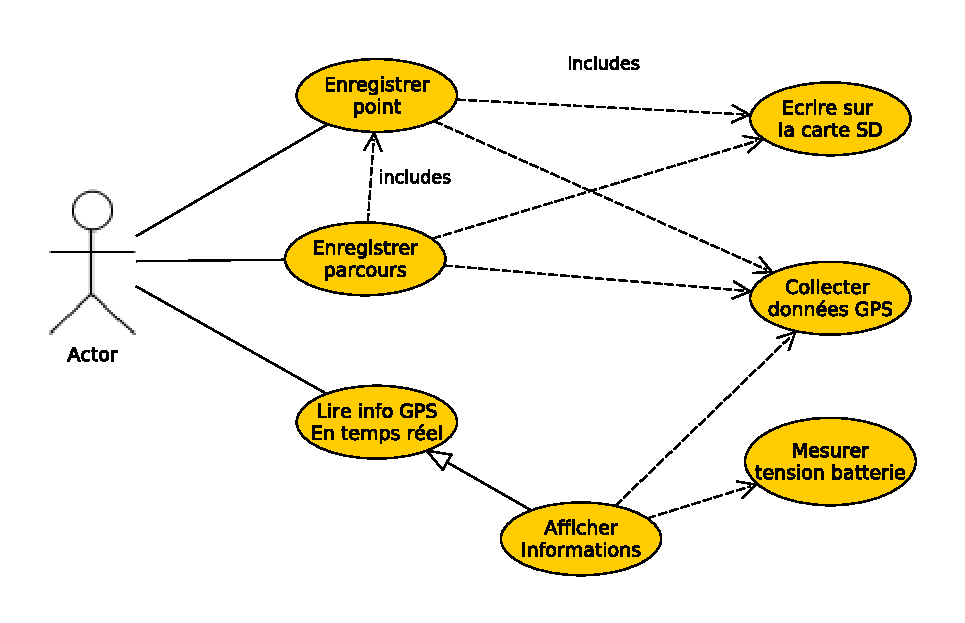
\includegraphics[scale = 0.9]{UseCase.eps}
		\caption{Diagramme de cas d'utilisation}
	\end{center}
\end{figure}
\FloatBarrier
\newpage
\section{Description fonctionnelle}
Pour nous faciliter le travail de dévelloppement, nous avons utilisé des bibliothèques de fonctions déjà existantes, dont voici la liste exhaustive:
\begin{itemize}
\item TinyGPS, bibliothèque de traitement de données brutes GPS
\item SoftwareSerial, pour effectuer la liaison serial avec le recepteur GPS
\item avr/pgmspace, permettant de stocker des variables dans la mémoire flash de l'arduino
\item Bounce2, pour éviter de capter les rebonds des boutons poussoir
\item LiquidCrystal, facilitant l'utilisation de l'écran LCD
\item SD, bibliothèque native d'Arduino permettant de créer des objets\\ ``File'' et de les enregistrer
\end{itemize}

Lors du dévellopement, nous avons décidé de découper notre programme en plusieurs ``bibliothèques'' de fonctions Arduino, chacune orientée sur un aspect du programme du système.
\subsection{Bibliothèque GPS}
Cette bibliothèque de fonctions nous permet de définir les variables globales liées au GPS (comme un booléen indiquant si les données GPS ont changé), ainsi que la fonction de mise à jour des coordonnées GPS. Cette dernière récupère toutes les données fournies par la bibliothèque TinyGPS, et les stocke dans un tableau.
\subsection{Bibliothèque d'affichage}
\subsection{Bibliothèque SD}
A partir de la bibliothèque native d'Arduino permettant d'écrire et lire sur une carte SD, nous avons codé des fonctions permettant d'écrire toutes les données GPS instantanées sur un fichier ou de lire un fichier et d'écrire son contenu sur le port série. Nous avions aussi prévu de lister les fichihers présent sur la carte SD, mais cette option n'a pas pu être implémentée faute de place sur l'Arduino.

En figure 2 se trouve l'algorithme de la fonction \textit{loop}. Les algorithmes des bibliothèques que nous avons dévelloppé ne sont pas détaillées ici, car il sont relativement simples et ne présentent pas grand intérêt.
\newpage
%\begin{landscape}
\begin{figure}[!ht]
	\begin{center}
		
		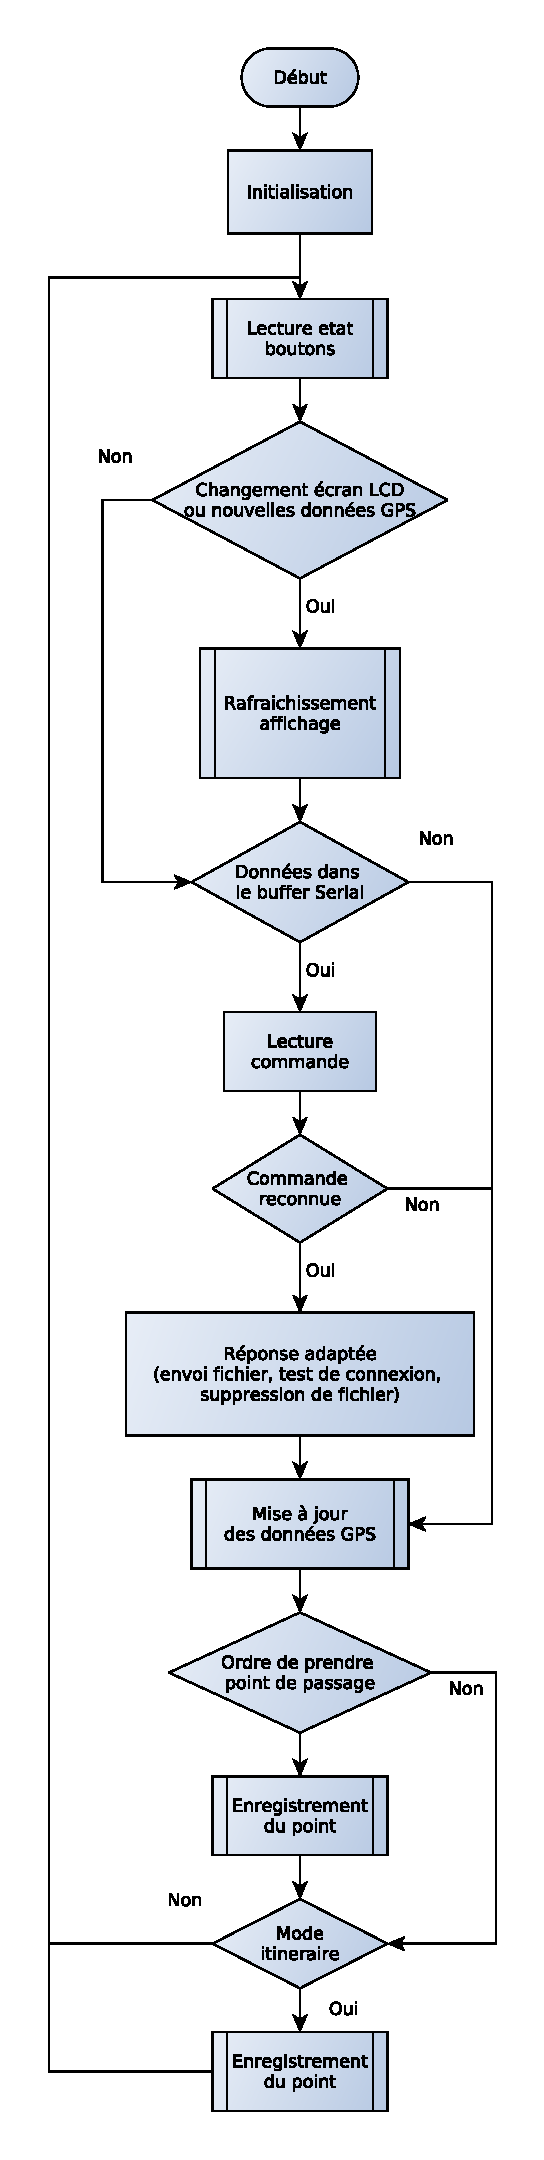
\includegraphics[scale = 0.5]{MainAlgoGraph.eps}
		\caption{Boucle principale}
	\end{center}
\end{figure}
\FloatBarrier
\newpage

\section{Traitement et interprétation des données}
Nous avons effectué 5 séries de mesures dans plusieurs lieux différents: Un appartement au dernier étage du centre ville de Troyes, une voiture à l'arrêt dans un parking, un appartement au premier étage d'uh immeuble, la terrasse de la salle associative de l'UTT (très proche d'une structure métallique) et une petite coline dégagée.
Le choix de ces endroits nous a semblé crucial car les mesures prises nous permettront d'estimer les paramètres influençant la précision du GPS.


\section*{Conclusion}

\end{document}
